\documentclass[12pt,a4paper]{article}
\usepackage[slovene]{babel}
\usepackage{amsmath}
\usepackage{amsfonts}
\usepackage{amssymb}
\usepackage{graphicx}
\usepackage{lmodern}
\usepackage{hyperref}
\usepackage{xcolor}
\usepackage{adjustbox}
\usepackage{multirow}
\usepackage[left=2cm,right=2cm,top=2cm,bottom=2cm]{geometry}
\author{Tina Zwittnig 64200432}
\title{Poročilo 5. vaje pri predmetu OVS \\ Sivinske preslikave slik}


\begin{document}
\maketitle
\pagebreak
\section{Minimalne in maksimalne sivinske vrednosti}
\begin{table}[h]
\centering
        \begin{tabular}{|c|c|c|c|c|}
      \hline
      vrsta preslikave & \multicolumn{2}{|l|}{V bazi int16 } & \multicolumn{2}{|l|}{V bazi uint8 } \tabularnewline
      \hline 
      vrednost & min vrednost & maks. vrednost &min vrednost & maks. vrednost\\
      \hline 
     originalna slika & -10128 & 455 & 0 & 255\\
      \hline
      linearna preslikava &199.1250 &1522 & 199 &255 \\
      \hline
      linearno oknjenje & 0 &255 &0 &255\\
      \hline
       odsekoma linearna & 2.4437 &  254.0225 &  2 & 254 \\
      \hline
      gamma preslikava & 0 &255 &0 & 255\\
      \hline
    \end{tabular}
%     \end{adjustbox}
%     \vspace{ - 05 mm}
    \caption{Tabela z minimalnimi in maksimalnimi vrednostmi}
    \label{tab:xxx}
\end{table}
\section{Upragovanje}
\begin{verbatim}
function oImage = thresholdImage(iImage, iT)
%trehsholdImage naredi upragovanje slike.
%vhodni parametri:
%   iImage  - slika podana v matrični obliki
%   iT - parameter upragovanja
%izhodni paramatri:
%   oImage - slika pridobljena z upragovanjem v matrični obliki.

    Lg = 2^8 -1;
    oImage = iImage;
    oImage(iImage<=iT) = 0;
    oImage(iImage>iT) = Lg;
end


\end{verbatim}
\section{Štetje sivinskih vrednosti $s_g = 0$}
S tem, ko upragujemo sliko pri nekem parametru $t$ v resnici izračunamo koliko sivinskih vrednosti je manjših ali enakih $t$. S tem vbistvu računamo komulativno ferkvenco. Za isto sliko sem izračunala tudi relativno komulativno ferkvenco, ki je ponazorena v drugem histogramu. Vidimo, da se obliki ujemata. Ker je ena relativna komulativna ferkvenca in ena ni relativna so vrednosti na y osi različne.
\pagebreak
\begin{figure}[h!]
  \begin{center}
    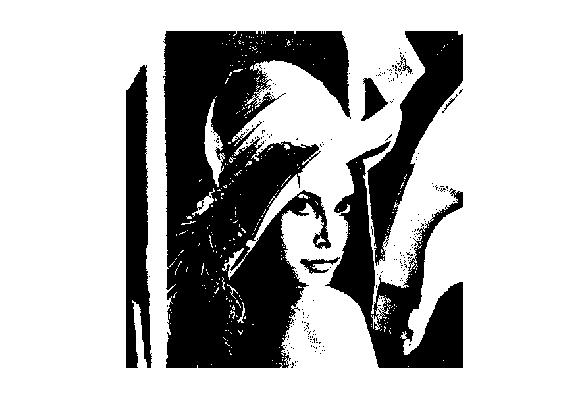
\includegraphics[scale = 0.7]{prag.jpg}
    \caption{Slika, ki jo dobimo če za upragovanje uporabimo parameter t = 127}
    \label{fig:}
  \end{center}
\end{figure}

\begin{figure}[h!]
  \begin{center}
    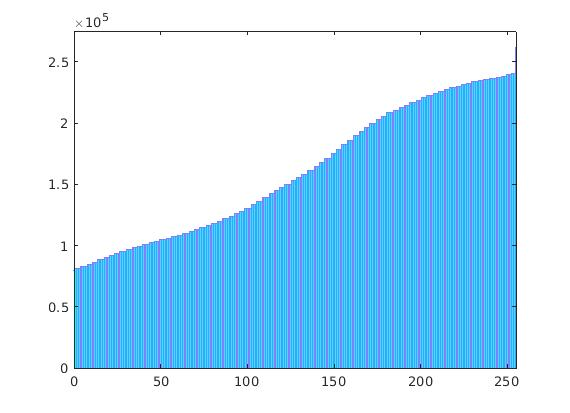
\includegraphics[scale = 0.7]{histogram1.jpg}
    \caption{Histogram, ki ponazarja, koliko je elementov $s_g = 0$, glede na paramater $t$}
    \label{fig:}
  \end{center}
\end{figure} 
\pagebreak
\begin{figure}
  \begin{center}
    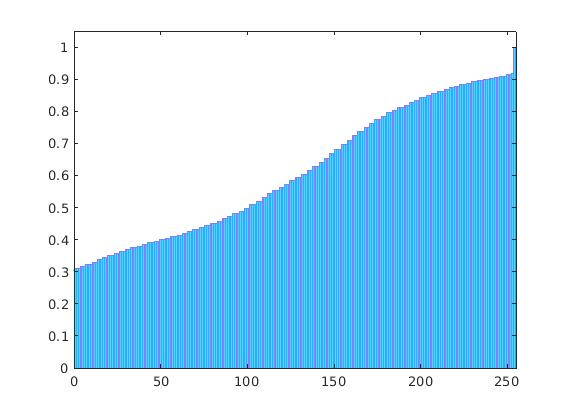
\includegraphics[scale = 0.7]{histogram2.jpg}
    \caption{Histogram relativne komulativne ferkvence slike}
    \label{fig:}
  \end{center}
\end{figure}
\begin{verbatim}
slika = loadImage('image-512x512-16bit.raw',[512,512], 'int16');
linearna = scaleImage(slika, -0.125, 256);
oknjenje = windowImage(linearna, 1000,500);
prikaz = displayImage(oknjenje, 'oknjenje');

sivniske = linspace(0,1, 256);
stevilo_nicel = zeros(1,256)
for prag = 0:255
    upragovana = thresholdImage(oknjenje, prag);
    indeksi = upragovana <= 0;
    stevilo_nicel(prag+1) = sum(indeksi(:));
end
displayHistogram(stevilo_nicel,sivniske,'Histogram, ki prikazuje število črnih elementov v sliki')
[hist, ~, cdf, levels] = computeHistogram(prikaz.CData)
displayHistogram(cdf,levels, 'komulativna ferkvenca');
\end{verbatim}
\pagebreak
\section{Odsekoma nelinearna preslikava}
\begin{verbatim}
function oImage = nonLinearSectionalScaleImage(iImage, iS, oS)
%nonLinearSectionalScaleImage naredi odsekoma nelinearno preslikavo z danimi parametri
%vhodni elementi:
%   iImage - vhodna slika v obliki matrike
%   iS - seznam x komponent kontrolnih točk
%   oS - seznam y komponent kontrolnih točk
%izhodni elementi
%   oImgae - preslikana slika

oImage = iImage;
for i = 1: 2:length(iS)-2
    Ax = iS(i);% tocka A
    Bx = iS(i+1);% tocka B
    Cx = iS(i+2); %tocka C
    sistem = [Ax^2 Ax 1;
              Bx^2 Bx 1;
              Cx^2 Cx 1]; % izračunane vrednosti za sistem enačb
   Ay = oS(i);
   By = oS(i+1);
   Cy = oS(i+2);
   Y = [Ay;
       By;
       Cy]; %Y komponente enačbe
   
   koeficienti = sistem\Y %rešimo sistem enačb
   
   i
   a1 = koeficienti(1)
   b1 = koeficienti(2)
   c1 = koeficienti(3)
   tmp = find(iImage>=Ax & iImage<=Cx);
   %kvadratna funkcija a1*x^2 + b1*x + c1
   oImage(tmp) = a1*iImage(tmp).^2 + b1 * iImage(tmp) +c1;
end
\end{verbatim}
\pagebreak
\begin{figure}
  \begin{center}
    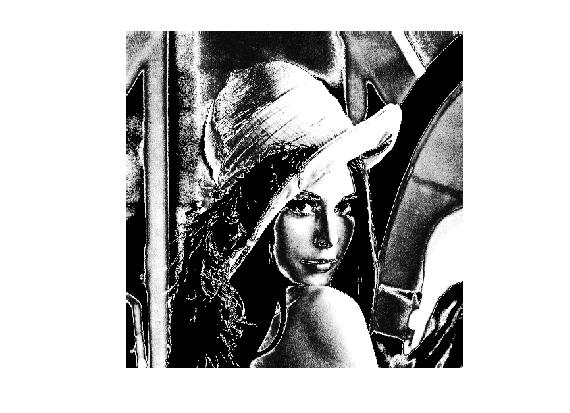
\includegraphics[scale = 0.7]{cetrta.jpg}
    \caption{Slika, ki jo dobimo, če sivinske vrednosti preslikamo z odsekoma nelinearno preslikavo}
    \label{fig:}
  \end{center}
\end{figure}

Pri odsekoma kvadratični preslikavi dobimo koeficiente polinoma:
\begin{table}[h]
\centering
        \begin{tabular}{|c|c|c|c|}
      \hline
      &$A_i$&$B_i$& $C_i$ \\
      \hline
      \hline
      $i= 1$ &-0.1344 &11.7500 &0\\
      \hline
      $i = 3$ &0.0569 &-13.0580&760.3830 \\
      \hline
      $i = 3$ &-0.0172 &    8.2531 &-731.9297\\
      \hline
      
      
      
    \end{tabular}

    \caption{Tabela z koeficienti kvadratne funkcije}
    \label{tab:xxx}
\end{table}
\end{document}
